\classheader{2018-08-21}
\subsection*{Homogeneous with constant coefficients}
Let $\vec{x}' = A_{nxn} \vec{x}, \quad$ $A_{nxn}$ - matrix of constants. (\textbf{Note:} $\vec{x}' = \begin{bmatrix}
			1 & 1\\ 6 & 0
		\end{bmatrix} \vec{x}$ is an example.)
For $n=2$, solutions look like $\vec{x}(t) = \begin{bmatrix}
	x_1(t)\\ x_2(t)
\end{bmatrix}$. For each $t$, $\vec{x}(t)$ is a point in $\mathbb{R}^2$. As $t$ evolves, $\vec{x}(t)$ will trace out a parameterized curve.
\begin{center}
	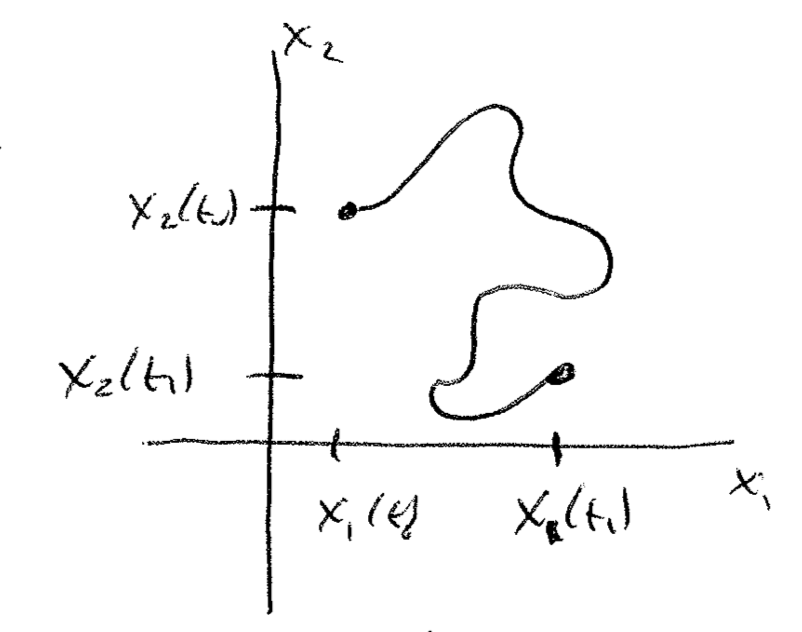
\includegraphics[scale=0.5]{22-1}
\end{center}
We call the $x_1, x_2$-plane the \underline{phase plane} for the system, noting that
\begin{enumerate}[label=\protect\circled{\alph*}]
	\item the independent variable $t$ is implicit to the graph (not an axis, but on the curve)
	\item For one equation $y' = f(y)$, the solution $y(t)$ lived in the $ty$-plane, but we could also track its evolution in the \underline{phase line}
	\item We could graph $\vec{x}(t)$ in the $tx_1 x_2$-space but this is hard to see.
\end{enumerate}
\subsubsection*{Some ideas for study}
\begin{enumerate}[label=\protect\circled{\Roman*}]
	\item $\vec{x}'(t) = A \vec{x}(t)$, by simply choosing points $\vec{x} \in \mathbb{R}^2$, we can plot tangent lines and make a slope field in the phase plane.
	\begin{example-N}
		Let $A = \begin{bmatrix}
			1 & 1\\ 6 & 0
		\end{bmatrix}$. Compute
		\begin{enumerate}[label=\protect\circled{\alph*}]
		\item $\vec{x} = \begin{bmatrix}
			1\\2
		\end{bmatrix}$, $\vec{x} = \begin{bmatrix}
			1 & 1\\ 6 & 0
		\end{bmatrix}
		\begin{bmatrix}
			1\\2
		\end{bmatrix} = 
		\begin{bmatrix}
			3\\6
		\end{bmatrix}$
		\item $\vec{x} = \begin{bmatrix}
			1\\0
		\end{bmatrix}$, $\vec{x} = \begin{bmatrix}
			1 & 1\\ 6 & 0
		\end{bmatrix}
		\begin{bmatrix}
			1\\0
		\end{bmatrix} = 
		\begin{bmatrix}
			1\\6
		\end{bmatrix}$\\
		\textbf{Notes: } 
			\begin{enumerate}[label=\protect\circled{\arabic*}]
			\item looks very similar to example 1
			\item Use JODE 2D calculator on website
			\end{enumerate}
	\end{enumerate}
	\end{example-N}
		\begin{center}
			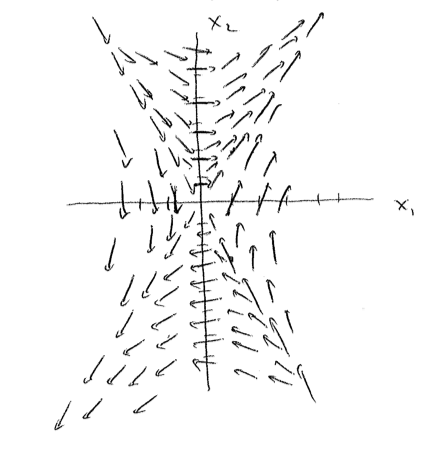
\includegraphics[scale=0.6]{22-2}
		\end{center}
	\item The solution curves will be integral curves of this slope field:
	\begin{enumerate}[label=\protect\circled{\alph*}]
	\item Given a value of $c_1, c_2 \in \mathbb{R}$, the curve $\vec{x(t)} = c_1 \begin{bmatrix}
				1\\2
			\end{bmatrix} e^{3t} + c_2
			\begin{bmatrix}
				1\\-3
			\end{bmatrix} e^{-2t}$ will be one of these curves.
	\item Straight line motion occurs when $c_1$ or $c_2 = 0$ 
	\end{enumerate}
\end{enumerate}
Choose $c_1 = -2, c_2 = 0$. then $\vec{x}(t) = -2 \begin{bmatrix}
	1\\2
\end{bmatrix} e^{3t} = \begin{bmatrix}
	-2\\-4
\end{bmatrix}e^{3t}$
\begin{center}
	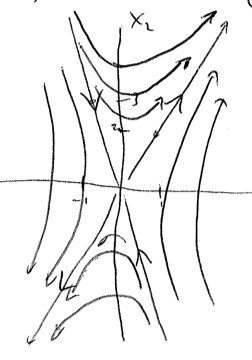
\includegraphics{22-3}
\end{center}